\begin{figure}[h]
\centering
\begin{minipage}[t]{0.48\columnwidth}
  \centering
  \vspace{0pt}
    \captionof{table}{Ablation study of whether using \\Complex Human Instruction (CHI).}
    \vspace{-0.5em}
    \label{tab:ablation_chi}
    \scalebox{0.9}{
    \begin{tabular}{lll}
    \toprule
    \textbf{Prompt} & \textbf{Train Step} & \textbf{GenEval} \\
    \midrule
    User & \multirow{2}{*}{52K} & 45.5 \\
    CHI + User & & 47.7~(+2.2) \\
    \midrule
    User & 140K & 52.8 \\
    CHI + User & + 5K(finetune) & 54.8~(+2.0) \\
    \bottomrule
    \end{tabular}
    }
\end{minipage}
\hfill
\begin{minipage}[t]{0.48\columnwidth}
  \centering
  \vspace{0pt}
    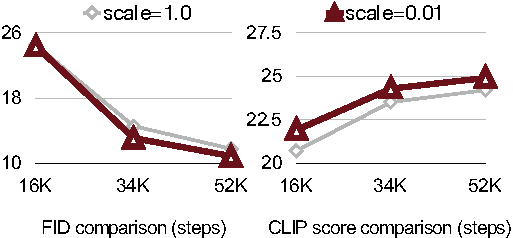
\includegraphics[width=0.9\textwidth]{figures/ablation_y_norm_scale_factor.pdf} 
    \vspace{-0.5em}
    \caption{Ablation study of whether using text embedding normalization and small scale factor. 
    }
    \label{fig:ablation_y_norm_sf}
\end{minipage}
\label{fig:combined}
\end{figure}